\documentclass[10pt]{beamer}
\usepackage[utf8]{inputenc}
\usepackage{graphicx}
\usepackage{mathtools}
\usetheme{CambridgeUS}
\usecolortheme{dolphin}
\usepackage{listings}
\usepackage{pdfpages}

% Set up hyperref once and configure colors
\usepackage{hyperref}
\hypersetup{
    colorlinks=true,
    linkcolor=blue,
    linktocpage=true
}

% Custom colors
\definecolor{myNewColorA}{RGB}{118,193,188}
\definecolor{myNewColorB}{RGB}{106,172,150}
\definecolor{myNewColorC}{RGB}{94,150,218}
\setbeamercolor*{palette primary}{bg=myNewColorC}
\setbeamercolor*{palette secondary}{bg=myNewColorB, fg=white}
\setbeamercolor*{palette tertiary}{bg=myNewColorA, fg=white}
\setbeamercolor*{titlelike}{fg=myNewColorA}
\setbeamercolor*{title}{bg=myNewColorA, fg=white}
\setbeamercolor*{item}{fg=myNewColorA}
\setbeamercolor*{caption name}{fg=myNewColorA}
\usefonttheme{professionalfonts}

\titlegraphic{
\includegraphics[height=1.5cm]{../CommonFigures/Universidad_Panamericana-logo.jpg}}

\setbeamerfont{title}{size=\large}
\setbeamerfont{subtitle}{size=\small}
\setbeamerfont{author}{size=\small}
\setbeamerfont{date}{size=\small}
\setbeamerfont{institute}{size=\small}
\title[Universidad Panamericana]{}
\subtitle{FreeRTOS Architecture Part 1}
\author[]{Name}
\institute[ltonix@up.edu.mx]{Universidad Panamericana}
\date[Presentation \today]{Presentation \today}

\AtBeginSection[]{
  \begin{frame}
  \vfill
  \centering
  \begin{beamercolorbox}[sep=8pt,center,shadow=true,rounded=true]{title}
    \usebeamerfont{title}\insertsectionhead\par%
  \end{beamercolorbox}
  \vfill
  \end{frame}
}

\setbeamercolor{block title}{bg=myNewColorA, fg=black} % Background and foreground colors for the block title
\setbeamercolor{block body}{bg=myNewColorC, fg=black} % Background and foreground colors for the block body

% Setup listings
\lstset{
  basicstyle=\ttfamily\small,
  keywordstyle=\color{blue},
  commentstyle=\color{green},
  stringstyle=\color{red},
  backgroundcolor=\color{gray!10},
  frame=single,
  language=C++,
  breaklines=true,
  showspaces=false,
  showstringspaces=false
}


\begin{document}

\frame{\titlepage}
\begin{frame}
\frametitle{Contents}
\tableofcontents
\end{frame}

\section{Why good practices?}
\begin{frame} {Why good practices?}
    \begin{itemize}
      \item \textbf{1. Maintainability}
      \begin{itemize}
        \item This is crucial for long-term projects where multiple developers might be working on the same codebase over time.
      \end{itemize}
      \item \textbf{2. Readability}
      \begin{itemize}
        \item Clear and consistent coding standards make it easier for developers to read and understand each other's code.
      \end{itemize}
      \item \textbf{3. Reusability}
      \begin{itemize}
        \item This means that code can be reused in different parts of a project or even in different projects, saving time and effort.
      \end{itemize}
      \item \textbf{4. Bug Reduction}
      \begin{itemize}
        \item Identifying and fixing bugs early in the development process.
      \end{itemize}
      \item \textbf{5. Performance}
      \begin{itemize}
        \item This is particularly important in applications where performance is critical, such as real-time systems or high-traffic web services.
      \end{itemize}
    \end{itemize}
  
\end{frame}

\begin{frame}{Why Good Practices?}
  \begin{itemize}
    \item \textbf{6. Scalability}
    \begin{itemize}
      \item Be easily extended with new features wiYout significant rework.
    \end{itemize}
    \item \textbf{7. Security}
    \begin{itemize}
      \item Secure data handling are crucial in preventing security breaches.
    \end{itemize}
    \item \textbf{8. Documentation}
    \begin{itemize}
      \item For future maintenance, debugging, and onboarding new developers.
    \end{itemize}
    \item \textbf{9. Consistency}
    \begin{itemize}
      \item It allows developers to switch between different parts of the codebase wiYout needing to adjust to different coding styles.
    \end{itemize}
    \item \textbf{10. Professionalism}
    \begin{itemize}
      \item It can enhance the reputation of a development team or company and build trust with clients and stakeholders.
    \end{itemize}
  \end{itemize}
\end{frame}


\begin{frame}{10 commandments}
  \begin{enumerate}
    \item \textbf{You shall prioritize Maintainability}
    \item \textbf{You shall value Readability}
    \item \textbf{You shall strive for Reusability}
    \item \textbf{You shall reduce Bugs early}
    \item \textbf{You shall optimize Performance}
    \item \textbf{You shall ensure Scalability}
    \item \textbf{You shall secure thy code}
    \item \textbf{You shall document thoroughly}
    \item \textbf{You shall maintain Consistency}
    \item \textbf{You shall uphold Professionalism}
  \end{enumerate}
\end{frame}



\section{Use other programming languages}
\begin{frame} {You shouldn't be opposed to learning programming languages.}
  \begin{itemize}
    \item Latex : Documentation
    \item Java: PlantUML
    \item JSON: For automatization stuff
    \item Python: Unit Testing
    \item C: Pretty basic programming
    \item Cpp: Robust programming
    \item C\#: Windows App
  \end{itemize}

\end{frame}

  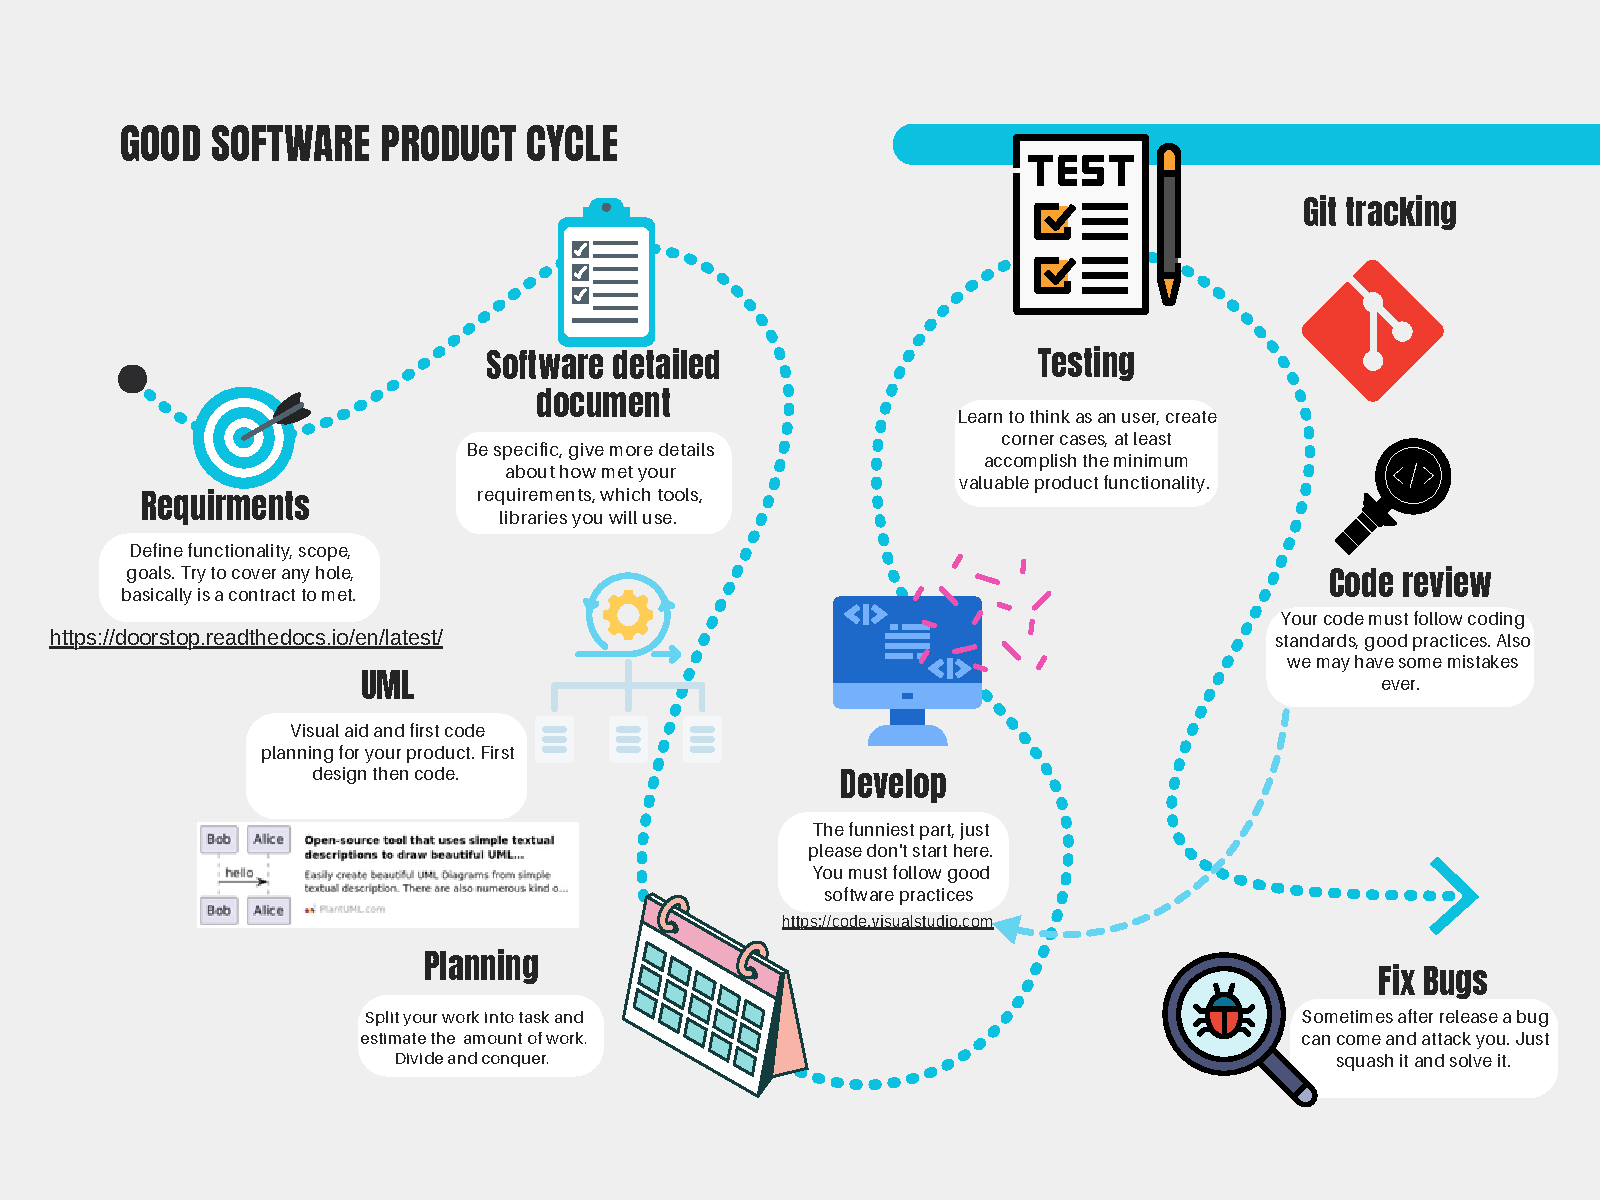
\includepdf{figures/SoftwareProductCycle.pdf}

\section{Requirements}
\begin{frame} {Requirements}

\end{frame}


\section{SDD}
\begin{frame} {Software Detailed Document (SDD)}

\end{frame}

\section{SDG}
\begin{frame} {Software Development Guide (SDG)}

\end{frame}


\section{UML}
\begin{frame} {Unified Modeling Language with PlantUML (UML)}
  UML diagrams serve as excellent documentation tools that are useful throughout the system's lifecycle. \
  They help new team members understand the system quickly and can also be valuable for maintenance and future upgrades.
\end{frame}


\section{Testing}
\begin{frame} {Black box vs Whitebox testing}

\end{frame}

\section{TPD}
\begin{frame} {Test plan document (TPD)}

\end{frame}




\end{document}